\documentclass[a4paper,11pt,DIV14,BCOR0mm]{scrartcl}
\usepackage[utf8]{inputenc}
\usepackage[francais]{babel}
\usepackage[T1]{fontenc}
\usepackage{amsmath}
\usepackage{amssymb}
\usepackage{color}
\usepackage{textcomp}
\usepackage[official]{eurosym}
\usepackage{enumitem}
\usepackage{numprint}
\usepackage{graphicx}
\usepackage{xifthen}
\usepackage{pifont}
%\usepackage{xlop}
\usepackage{subfig}
\usepackage{cellspace,stmaryrd}
\usepackage[french]{varioref}
\usepackage{pstricks,pst-circ,pstricks-add,pst-plot,pst-math}
%\usepackage{pst-all,pst-tree,pst-3dplot}
\RequirePackage[amsmath,thmmarks,hyperref,framed]{ntheorem}
\usepackage{mathrsfs}

% ==================================================
% Intervalles
% ==================================================
\newcommand{\intervalle}[4]{\mathopen{#1}#2\mathpunct{};#3\mathclose{#4}}
\newcommand{\intff}[2]{\intervalle{[}{#1}{#2}{]}}
\newcommand{\intof}[2]{\intervalle{]}{#1}{#2}{]}}
\newcommand{\intfo}[2]{\intervalle{[}{#1}{#2}{[}}
\newcommand{\intoo}[2]{\intervalle{]}{#1}{#2}{[}}
\newcommand{\intn}[2]{\intervalle{\llbracket}{#1}{#2}{\rrbracket}}
\newcommand{\bigintervalle}[4]{\bigl{#1}#2\mathpunct{};#3\bigr{#4}}
\newcommand{\bigintff}[2]{\bigintervalle{[}{#1}{#2}{]}}
\newcommand{\bigintof}[2]{\bigintervalle{]}{#1}{#2}{]}}
\newcommand{\bigintfo}[2]{\bigintervalle{[}{#1}{#2}{[}}
\newcommand{\bigintoo}[2]{\bigintervalle{]}{#1}{#2}{[}}
\newcommand{\bigintn}[2]{\bigintervalle{\llbracket}{#1}{#2}{\rrbracket}}
\newcommand{\Bigintervalle}[4]{\Bigl{#1}#2\mathpunct{};#3\Bigr{#4}}
\newcommand{\Bigintff}[2]{\Bigintervalle{[}{#1}{#2}{]}}
\newcommand{\Bigintof}[2]{\Bigintervalle{]}{#1}{#2}{]}}
\newcommand{\Bigintfo}[2]{\Bigintervalle{[}{#1}{#2}{[}}
\newcommand{\Bigintoo}[2]{\Bigintervalle{]}{#1}{#2}{[}}
\newcommand{\Bigintn}[2]{\Bigintervalle{\llbracket}{#1}{#2}{\rrbracket}}
\newcommand{\biggintervalle}[4]{\biggl{#1}#2\mathpunct{};#3\biggr{#4}}
\newcommand{\biggintff}[2]{\biggintervalle{[}{#1}{#2}{]}}
\newcommand{\biggintof}[2]{\biggintervalle{]}{#1}{#2}{]}}
\newcommand{\biggintfo}[2]{\biggintervalle{[}{#1}{#2}{[}}
\newcommand{\biggintoo}[2]{\biggintervalle{]}{#1}{#2}{[}}
\newcommand{\biggintn}[2]{\biggintervalle{\llbracket}{#1}{#2}{\rrbracket}}
\newcommand{\Biggintervalle}[4]{\Biggl{#1}#2\mathpunct{};#3\Biggr{#4}}
\newcommand{\Biggintff}[2]{\Biggintervalle{[}{#1}{#2}{]}}
\newcommand{\Biggintof}[2]{\Biggintervalle{]}{#1}{#2}{]}}
\newcommand{\Biggintfo}[2]{\Biggintervalle{[}{#1}{#2}{[}}
\newcommand{\Biggintoo}[2]{\Biggintervalle{]}{#1}{#2}{[}}
\newcommand{\Biggintn}[2]{\Biggintervalle{\llbracket}{#1}{#2}{\rrbracket}}

\newcommand{\pt}{.}
\newcommand{\et}{\text{ et }}
\newcommand{\si}{\text{ si }}
\newcommand{\tq}{\text{ tq }}
\newcommand{\sinon}{\text{ sinon }}
\newcommand{\avec}{\text{ avec }}
\def\pour{\text{~pour~}}

\newenvironment{enumeratecol}[1][2]{\begin{multicols}{#1}\begin{enumerate}}{\end{enumerate}\end{multicols}}


\newcommand{\set}[1]{\left\{#1\right\}}


%\newtheorem{theoreme}{Théorème}
%\newtheorem{axiome}{Axiome}
\newtheorem*{proprieteadmise}{Propriété (admise)}
%\newtheorem*{demonstration}{Démonstration}
\newtheorem*{notation}{Notation}
\newtheorem*{application}{Application}
\newtheorem*{consequence}{Conséquence}
\newtheorem{roc}{Restitution organisée de connaissances.}


\theoremstyle{plain}
\theoremheaderfont{\normalfont\bfseries}
\theorembodyfont{\normalfont}
\theoremseparator{.}
\newtheorem{exercice}{Exercice}
\newtheorem{cours}{Question de cours}
\newtheorem{probleme}{Problème}

\theoremstyle{plain}
\theoremheaderfont{\normalfont\bfseries}
\theorembodyfont{\normalfont}
\theoremseparator{.}
\newtheorem*{rappel}{Rappel}
\newtheorem{exemple}{Exemple}
\newtheorem*{contreexemple}{Contre-exemple}
\newtheorem{remarque}{Remarque}
\newtheorem*{interpretation}{Interprétation}
\newtheorem*{convention}{Convention}
\newtheorem*{vocabulaire}{vocabulaire}

\theoremheaderfont{\sc}\theorembodyfont{\upshape}
\theoremstyle{nonumberplain}
\theoremseparator{ : }
%\theoremsymbol{\rule{1ex}{1ex}}
\theoremsymbol{\ensuremath\square}
\newtheorem{demonstration}{D\'emonstration}



\usepackage[S]{thmbox}
\newtheorem[S]{theoreme}{Théorème}
\newtheorem[S]{propriete}{Propriété}
\newtheorem[S]{axiome}{Axiome}
\newtheorem[S]{methode}{Méthode de résolution}
\newtheorem[L]{definition}{Définition}

\newcommand{\defi}[1]{
\begin{definition}
#1
\end{definition}
}

\newcommand{\theo}[1]{
\begin{theoreme}
#1
\end{theoreme}
}

\newcommand{\demo}[1]{
\begin{demonstration}
#1
\end{demonstration}
}


%-------------------------------------------------
%         TYPOGRAPHIE
%-------------------------------------------------
\newcommand{\celsius}{\,\degres\textrm{C}}


%-------------------------------------------------
%         SCOLAIRE
%-------------------------------------------------
\newcommand{\trou}[1]{\textcolor{white}{#1}}
\newcommand{\prof}[1]{\textcolor{blue}{#1}}
\newcommand{\exercices}[1]{\begin{flushright}\textbf{Exercices : }#1\end{flushright}}

\newcommand{\np}[1]{\numprint{#1}}

\newcommand{\place}[1]{
\vfill\begin{center}
< #1>
\end{center}
\vfill
}

\newif\ifeleve
\def\ac#1{\ifeleve%
\setbox1\hbox{#1}%
\lower2pt\hbox to \wd1{\dotfill}%
\else#1\fi}

\newcommand{\croi}{% croissante
\unitlength=1cm
\begin{minipage} {1cm}%pour centrer verticalement f(x)
\begin{picture}(1,1) % dessin de 2 X 2
\put(0,0){\vector(1,1){1}} % 1 à partir (0,0) direction (1,1)
\end{picture}
\end{minipage}
}
\newcommand{\dec}{%décroissante
\unitlength=1cm
\begin{minipage} {1cm}%pour centrer verticalement f(x)
\begin{picture}(1,1) % dessin de 2 X 2
\put(0,1){\vector(1,-1){1}}
\end{picture}
\end{minipage}
} 

\newcommand{\tauxfxh}[3]{\dfrac{#1(#2+#3)-#1(#2)}{#3}}

\newcounter{QCM}
\setcounter{QCM}{1}
\newcommand{\question}[1]{{\item[Question \arabic{QCM}]\addtocounter{QCM}{1}#1}}
\newcommand{\choix}[3]{
\[
 \begin{tabular}{p{5cm}p{5cm}p{5cm}}
  \textbf{a) }#1.&\textbf{b) }#2.&\textbf{c) }#3.
 \end{tabular}
\]
}

%-------------------------------------------------
%         GEOMETRIE
%-------------------------------------------------
\newcommand{\vect}{\overrightarrow}
\newcommand{\norme}[1]{\|#1\|}
\newcommand{\Norme}[1]{\left\|#1\right\|}
\newcommand{\Oijk}{(O,\vect{i},\vect{j},\vect{k})}
\newcommand{\Oij}{(O,\vect{i},\vect{j})}
\newcommand{\Ouv}{(O,\vect{u},\vect{v})}
\newcommand{\bary}{\mathrm{Bar}}

%-------------------------------------------------
%         FONCTIONS
%-------------------------------------------------
\newcommand{\donne}{\mapsto}
\newcommand{\dx}{\mathrm{d}x}
\newcommand{\dt}{\mathrm{d}t}
\newcommand{\intab}{\int_{a}^{b}}
%-------------------------------------------------
%         PROBA
%-------------------------------------------------
\newcommand{\barre}[1]{\overline{#1}}

%-------------------------------------------------
%         ALGEBRE LINEAIRE
%-------------------------------------------------
\newcommand{\rg}{\text{rg}}
\newcommand{\tr}{\text{tr}}
\renewcommand{\Im}{\text{Im}}
\newcommand{\Vect}{\text{Vect}}
\newcommand{\LL}{\mathcal{L}}
\newcommand{\FF}{\mathcal{F}}
\newcommand{\MM}{\mathcal{M}}
\newcommand{\transpose}{{}^{t}}
%\newcommand{\ker}{\text{ker}}
\newcommand{\coordo}[2]{
\begin{pmatrix}
#1 \\ #2
\end{pmatrix}
}

%-------------------------------------------------
%         ARITHMETIQUE
%-------------------------------------------------
\newcommand{\congru}{\equiv}

%-------------------------------------------------
%         NOMBRES COMPLEXES
%-------------------------------------------------
\newcommand{\e}{\mathrm{e}}
\newcommand{\ii}{\mathrm{i}}
\newcommand{\ei}[1]{\mathrm{e}^{\ii#1}}
\newcommand{\C}{\mathbb{C}}
\newcommand{\U}{\mathbb{U}}
\newcommand{\re}[1]{\mathrm{Re}(#1)}
\newcommand{\im}[1]{\mathrm{Im}(#1)}
\newcommand{\conj}[1]{\overline{#1}}
\newcommand{\abs}[1]{\left\lvert#1\right\rvert}
\renewcommand{\arg}[1]{\mathrm{Arg}(#1)}

\newcommand{\pparmin}[2]{\binom{#2}{#1}}
\newcommand{\Pparmin}[2]{\dbinom{#2}{#1}}

\newcommand{\R}{\mathbb{R}}
\newcommand{\K}{\mathbb{K}}
\newcommand{\N}{\mathbb{N}}
\newcommand{\Z}{\mathbb{Z}}
\newcommand{\D}{\mathbb{D}}
\newcommand{\Q}{\mathbb{Q}}
\newcommand{\rond}{\circ}
\newcommand{\repereoij}{repère orthonormal $(O,\vect{i},\vect{j})$}
\newcommand{\repereoijdirect}{repère orthonormal direct $(O,\vect{i},\vect{j})$}
\newcommand{\accoladedouble}[2]{\left\{\begin{array}{ll}#1\\#2\end{array}\right.}
\newcommand{\soitlasuite}[4]{Soit $(#1)$ la suite définie par $\accoladedouble{#2}{#3\text{ pour tout $#4$}}$}
\newcommand{\coordvect}[2]{\left(\begin{array}{c}#1\\#2\end{array}\right)}
\newcommand{\baremeexo}[1]{\marginpar{\textbf{(#1)}}}
\newcommand{\baremeque}[1]{\marginpar{(#1)}}
\newcommand{\bq}[1]{\marginpar{\textcolor{red}{(#1)}}}


\newcommand{\less}{\leqslant}
\newcommand{\more}{\geqslant}
\newcommand{\equi}{\Longleftrightarrow}
\newcommand{\implique}{\Rightarrow}
\newcommand{\equidef}{\stackrel{def}{\Longleftrightarrow}}
\newcommand{\ssi}{\Longleftrightarrow}
\newcommand{\eqdef}{\stackrel{def}{=}}
\newcommand{\egaldef}{\stackrel{\tiny{def}}{=}}
\newcommand{\egalnot}{\stackrel{\tiny{notation}}{=}}
\newcommand{\latin}[1]{\emph{#1}}
\newcommand{\negl}[1]{\underset{\text{\tiny{$#1$}}}{\ll}}

\newcommand{\limsuite}{\displaystyle\lim_{n\to+\infty}}

% Partie à ommettre en première lecture
\newcommand{\optionnel}[1]{\noindent\hrulefill \rotatebox{180}{\ding{72}\ding{72}\ding{72}} \hrulefill #1 \noindent\hrulefill \ding{72}\ding{72}\ding{72} \hrulefill}
% En tête et pieds custom
\usepackage{fancyhdr}
\pagestyle{fancy}
\lhead{\today}
\rhead{Cours}		
\lfoot{\tiny{vg}}
\cfoot{}
\rfoot{\tiny{Lycée Émile Loubet, Valence}}


% de Dupuy de lome
%\newcommand{\norme}[1]{\left\lVert\ifempty{#1}{\dotpourvariable}{#1}\right\rVert}
\newcommand{\bignorme}[1]{\bigl\lVert#1\bigr\rVert}
\usepackage{hyperref}
\rhead{Janvier - février 2012}
\chead{}
\lhead{Limites de suites}
\lfoot{\tiny{vg}}
\cfoot{\thepage}
\rfoot{\tiny{Julie-Victoire Daubié, Argenteuil, TS2}}
\begin{document}
\section{Rappels}

\subsection{Suites convergentes}
\begin{definition}
 Soit $(u_n)$ une suite numérique réelle et $\ell$ un réel. Lorsque tout intervalle ouvert contenant $\ell$
contient tous les termes de la suite à partir d'un certain rang, on dit que $(u_n)$ converge vers $\ell$ et
on note :
\[
 \lim_{n\to+\infty}u_n=\ell.
\]
\end{definition}
\begin{exemple}
 On a $
 \lim 5+\frac{1}{n}=5.
$
Mais considérons la suite $(u_n)_{n\in\N^*}$ définie par \[
 u_n=5+\frac{1}{n}+(10^{-9}+(-1)^n\times 10^{-9}).
\]
Elle ne ne converge pas : lorsque $n> 10^{10}$, le neuvième chiffre après la virgule alterne entre
0 et 2 : les termes de la suite ne peuvent pas tous être dans aucun intervalle ouvert
de diamètre plus petit que $10^{-9}$ par exemple.
\end{exemple}


\subsection{Suites tendant vers $+\infty$ ou $-\infty$.}
\begin{definition}
 Soit $(u_n)$ une suite numérique. Lorsque pour tout nombre réel $M$ il existe un rang à partir duquel 
tous les termes de la suite sont supérieurs
à $M$, on dit que $(u_n)$ tends vers $+\infty$ et on note :
\[
 \lim_{n\to+\infty}u_n=+\infty.
\]
\end{definition}

\begin{definition}
 Soit $(u_n)$ une suite numérique. Lorsque pour tout nombre réel $m$ il existe un rang à 
partir duquel tous les termes de la suite sont inférieurs
à $m$, on dit que $u_n$ tends vers $-\infty$ et on note :
\[
 \lim_{n\to+\infty}u_n=-\infty.
\]
\end{definition}

\begin{theoreme}[Admis, peut être pris comme axiome]
Une suite numérique réelle croissante et majorée converge dans $\R$.
\end{theoreme}
\begin{remarque}
 L'énoncé : \og une suite numérique rationnelle croissante et majorée converge dans $\Q$\fg{} est
faux. Par exemple, si $(u_n)$ est la suite des approximations décimales à $10^{-n}$ près de
$\sqrt{2}$ c'est une suite croissante majorée de décimaux donc de rationnels, qui converge mais pas
dans $\Q$ : dans $\R$.
\end{remarque}

De manière analogue, une suite décroissante et minorée converge dans $R$.
\begin{theoreme}
 Une suite croissante non majorée tend vers $+\infty$.
\end{theoreme}
\begin{demonstration}[à connaître]
 Soit $(u_n)$ une suite croissante non majorée. Soit $M$ un réel. Comme $M$ n'est pas un majorant
de $(u_n)$, il existe un rang $n_0$ tel que $u_{n_0}$ soit supérieur à $M$. 
Comme $(u_n)$ est croissante, à partir du rang $n_0$ tous les termes de
$(u_n)$ sont supérieurs à $u_{n_0}$ et donc à $M$. On a bien démontré que $(u_n)$ tends vers 
$+\infty$, puisque pour tout nombre réel $M$, on a déterminé un rang à partir duquel tous les termes de
la suite sont supérieurs à $M$.
\end{demonstration}
On démontre bien sûr de manière analogue qu'une suite décroissante minorée tend vers $-\infty$.
\begin{exemple}
 Une suite bornée qui ne converge pas : $u_n=(-1)^n$.
\end{exemple}
\begin{exemple}
 Une suite strictement croissante qui ne tend pas vers $+\infty$ : $u_n=1-\dfrac1n$.
\end{exemple}
\begin{exemple}
 Une suite non majorée qui ne tend pas vers $+\infty$ : $u_n=(-1)^nn$.
\end{exemple}

\subsection{Limites connues}
\begin{theoreme}[Admis, vu en première]
 \begin{enumerate}
  \item Pour tout entier $k$ supérieur à 1, $\displaystyle\lim_{n\to+\infty}n^k=+\infty$.
  \item $\displaystyle\lim_{n\to+\infty}\sqrt{n}=+\infty$.
  \item Soit $q$ un réel, alors :
      \begin{enumerate}
	\item si $\abs{q}<1$, alors $\displaystyle\lim_{n\to+\infty}q^n=0$,
	\item si $q>1$, alors $\displaystyle\lim_{n\to+\infty}q^n=+\infty$.
      \end{enumerate}
 \end{enumerate}
\end{theoreme}


\subsection{Opérations et limites}
On note $0^+$ la limite 0 par valeurs positives (la suite tend vers 0 et 
est positive à partir d'un certain rang) et $0^-$ la limite 0 par valeurs négatives.
\begin{theoreme}[Admis]
\begin{enumerate}
 \item Le passage à la limite commute avec les opérations sur les nombres réels
lorsqu'elles sont définies.
  \item Lorsqu'elles ne sont pas définies, elles commutent dans certains cas avec les conventions de prolongement 
des opérations :
  \begin{enumerate}
   \item Pour tout réel $\ell$,\begin{align*}
	  \ell+\infty&=+\infty,&\ell-\infty&=-\infty,&\frac{\ell}{+\infty}=\frac{\ell}{-\infty}&=0.
	  \end{align*}
   \item Pour tout réel $\ell>0$, ou pour $\ell=+\infty$ :\begin{align*}
	  \ell\times(+\infty)&=+\infty,&\ell\times(-\infty)&=-\infty,
			  &\frac{\ell}{0^+}&=+\infty,&\frac{\ell}{0^-}&=-\infty.
	  \end{align*}
    \item Pour tout réel $\ell<0$, ou pour $\ell=-\infty$ :\begin{align*}
	  \ell\times(+\infty)&=-\infty,&\ell\times(-\infty)&=+\infty,
			  &\frac{\ell}{0^+}&=-\infty,&\frac{\ell}{0^-}&=+\infty.
	  \end{align*}
  \end{enumerate}
  \item On ne peut pas adopter de convention pour les cas suivants car ils sont indéterminés\footnote{tout est possible
    selon les cas particuliers : limite finie,
    limite infinie, pas de limite.} :
    \begin{align*}
    +\infty-\infty&&0\times\infty&&\frac{\infty}{\infty}&&\frac{0}{0}
\end{align*}
\end{enumerate}
\end{theoreme}

\subsection{Comparaison et limites}
\begin{theoreme}[admis, théorème \og des gendarmes\fg]
 Soit $(a_n)$, $(b_n)$ et $(u_n)$ trois suites, et $\ell$ un réel tels que :
\begin{enumerate}
 \item \`A partir d'un certain rang, $a_n\leq u_n\leq b_n$.
 \item $\displaystyle\lim a_n=\lim b_n=\ell$.
\end{enumerate}
Alors $\displaystyle\lim u_n=\ell$.
\end{theoreme}

\section{Suites adjacentes}
\subsection{Définition}
\begin{definition}
 On dit que deux suites réelles $(u_n)$ et $(v_n)$ sont adjacentes lorsqu'elles
vérifient les 3 propriétés :
\begin{enumerate}
 \item pour tout $n\in \N$, $u_n\leq v_n$,
 \item la suite $(u_n)$ est croissante et la suite $(v_n)$ est décroissante,
  \item $\displaystyle\lim_{n\to+\infty}v_n-u_n=0$.
\end{enumerate}
\end{definition}
\vspace{1cm}
\hfill \trou{<dessins>} \hfill
\vfill
\vspace{1cm}
\begin{remarque}
 La propriété 1 est une conséquence des deux suivantes. C'est donc une aussi mauvaise définition
que de définir le rectangle comme un quadrilatère qui a quatre angles droits. 
\end{remarque}

\begin{theoreme}[admis]
 Deux suites $(u_n)$ et $(v_n)$ sont adjacentes si et seulement si 
elles vérifient les deux propriétés :
\begin{enumerate}
 \item la suite $(u_n)$ est croissante et la suite $(v_n)$ est décroissante,
  \item $\displaystyle\lim_{n\to+\infty}v_n-u_n=0$.
\end{enumerate}
\end{theoreme}

\subsection{Théorème des suites adjacentes}
\begin{theoreme}
 Si deux suites sont adjacentes, alors elles convergent vers une même limite.
\end{theoreme}
\begin{demonstration}
 Soit $(u_n)$ et $(v_n)$ deux suites adjacentes. Alors $(u_n)$ est majorée par 
$v_0$. En effet, comme $(v_n)$ est décroissante, on a, pour tout $n\in\N$ :
\[
 u_n\leq v_n \leq v_0.
\]
Donc $(u_n)$ est croissante et majorée, donc elle converge vers un réel $\ell$.
De manière analogue, on montre que $(v_n)$ est décroissante et minorée par
$u_0$, ce qui prouve qu'elle converve vers un réel que l'on note $\ell'$.
On a donc d'après les règle opératoires sur les limites $\displaystyle\lim_{n\to+\infty}v_n-u_n=l'-l$.
Or cette limite est nulle, d'o\`u $\ell=\ell'$.
\end{demonstration}
\pagebreak
\subsection{Deux exemples fondamentaux}
\subsubsection{Mesure d'aire}
On veut mesurer l'aire délimitée par l'ellipse :
\[
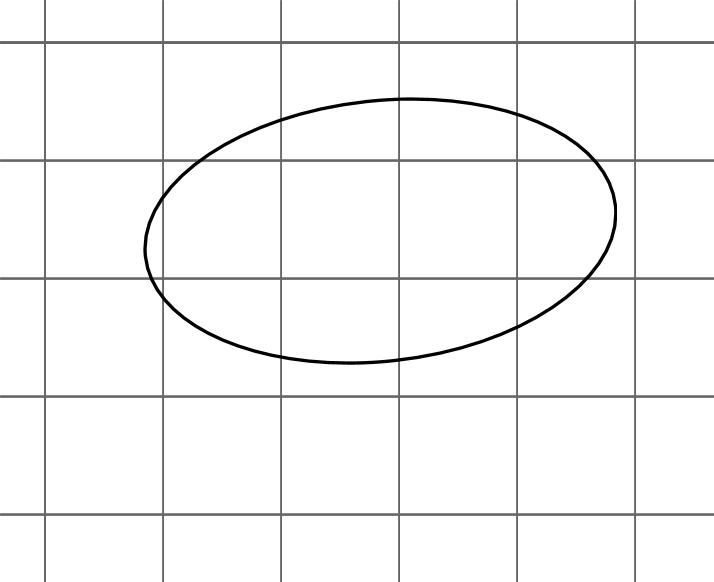
\includegraphics{aire1.png}\qquad\qquad\qquad\qquad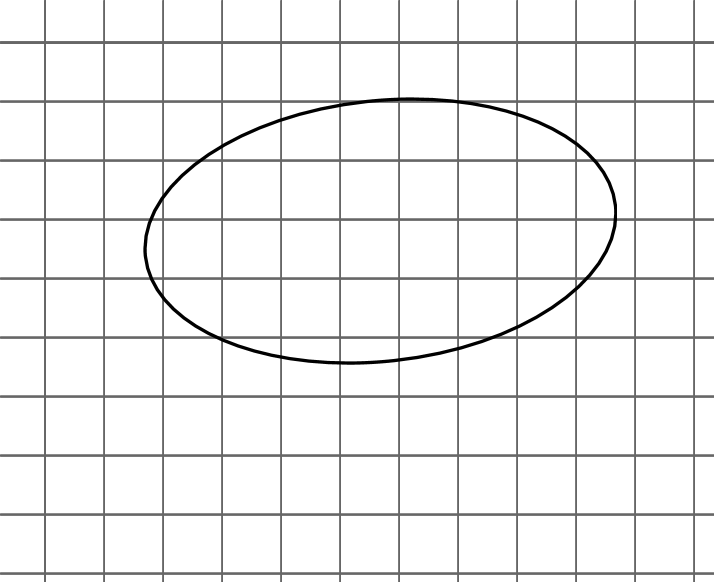
\includegraphics{aire2.png}
\]
\vfill

\subsubsection{Dichotomie}
Pour résoudre $\e^x=2$, on définit $f$ sur $\R$ par $f(x)=\e^x-2$, tableau de variation immmédiat. 
On cherche des valeurs approchées de $\alpha$ par dichotomie. Cela conduit à construire deux suites
$(a_n)$ et $(b_n)$ adjacentes :
\renewcommand{\arraystretch}{2}
\[\qquad\qquad\qquad\qquad\qquad\qquad\qquad\qquad
 \begin{array}{c|c|c|c|c}
  n	&	(a_n)	&	(b_n)	&	\trou{\dfrac{a_n+b_n}{2}}	&	\trou{f(\dfrac{a_n+b_n}{2})}\\\hline
  0	&	0	&	1	&	\trou{\dfrac{1}{2}}		&	\trou{-}\\\hline
  1	&\trou{\dfrac{1}{2}}	&	\trou{1}	&	\trou{\dfrac{3}{4}}		&	\trou{+}\\\hline
  2	&\trou{\dfrac{1}{2}}	&\trou{\dfrac{3}{4}}	&	\trou{\dfrac{5}{8}}		&	\trou{-}\\\hline
  3	&\dots		&\dots		&	\dots			&	\dots
 \end{array}
\]
La suite $(a_n)$ est croissante, la suite $(b_n)$ est décroissante, et comme $b_n-a_n=\trou{\left(\dfrac{1}{2}\right)^n}$,
on a bien $\displaystyle\lim_{n\to +\infty}b_n-a_n=0$.
\pagebreak

\section{Suites $u_{n+1}=f(u_n)$, théorème du point fixe}

\begin{theoreme}
 Soit $(u_n)$ une suite dé finie par $u_0=a$ et $u_{n+1}=f(u_n)$.
Si $(u_n)$ converge vers une limite $\ell$ et que $f$ est continue en $\ell$,
alors $\ell$ est une solution de l'équation $f(\ell)=\ell$.
\end{theoreme}


\end{document}
